\documentclass[11pt]{article}
\usepackage[margin=1in]{geometry}
\usepackage{amsmath, amssymb, amsthm}
\usepackage{booktabs}
\usepackage{graphicx}
\usepackage{hyperref}
\usepackage{natbib}
\usepackage{microtype}
\usepackage{xcolor}

\title{A Statistical Audit of LLM Calibration Heterogeneity\\Across Knowledge Domains}
\author{Jennifer Zhang \and John Wright}
\date{STAT 215B, Spring 2026}

\begin{document}
\maketitle

\begin{abstract}
Large language model (LLM) calibration is nearly always reported as a single
aggregate scalar, obscuring whether miscalibration is diffuse or concentrated
in specific knowledge domains. We develop a statistically rigorous audit
framework and apply it to MMLU \citep{hendrycks2021measuring} using token-level
log probabilities from four instruction-tuned models spanning two families and
three parameter scales: GPT-4o-mini, Llama-3-8B-Instruct,
Qwen-2.5-1.5B-Instruct, and Qwen-2.5-7B-Instruct. Our framework combines a
three-level mixed-effects model, isotonic and kernel-smoothed reliability
curves, empirical Bayes shrinkage, and Benjamini--Hochberg FDR correction.
Across all four models, between-subject calibration variance accounts for
1.9--7.9\% of the total, and 54--57 of 57 subjects are flagged as significantly
miscalibrated at FDR $\alpha=0.05$. Subject-level ECE rankings are highly
correlated across all model pairs (Spearman $\rho$ between 0.78 and 0.92),
indicating that miscalibration is task-driven rather than model-specific. The
same subjects are robustly worst-calibrated across the four models (college-level
quantitative STEM, niche factual recall, and structured ethical/legal
reasoning) and the same subjects are robustly best-calibrated (high-school-level
content in Social Sciences and applied/factual subjects). Question-level
entropy enters the multilevel model with a coefficient that varies in sign
across the four checkpoints---positive for GPT-4o-mini and Qwen-7B, marginal
for Llama, negative for Qwen-1.5B---a marginal pattern consistent with prior
aggregate findings on RLHF-induced confidence saturation
\citep{kadavath2022language, nakkiran2025trained}.
\end{abstract}

% ============================================================
\section{Introduction}
% ============================================================

Large language models are increasingly deployed in high-stakes settings---healthcare,
law, education---where the reliability of model-expressed confidence is as important as
accuracy itself. A well-calibrated model is one whose stated confidence tracks its
empirical accuracy: if a model assigns 80\% probability to an answer, it should be
correct 80\% of the time. Miscalibration, particularly overconfidence, means that users
who rely on model confidence as a decision signal will be systematically misled.

A substantial literature has studied LLM calibration. \citet{guo2017calibration}
established the modern empirical study of neural network calibration, popularizing
expected calibration error (ECE) as a standard metric and demonstrating the
effectiveness of temperature scaling as a post-hoc correction.
\citet{kadavath2022language} showed that for multiple-choice tasks, token-level log
probabilities provide a meaningful calibration signal, and that base (pre-RLHF) models
exhibit better-calibrated token probabilities than instruction-tuned counterparts.
\citet{xiong2024can} provided a systematic benchmark of confidence elicitation methods,
finding that all methods ``struggle in challenging tasks, such as those requiring
professional knowledge''---suggesting calibration quality may vary by domain, though the
authors do not investigate this directly. \citet{jiang2021can} similarly found that
question-level features such as answer entropy predict calibration quality, a pattern we
examine formally here.

What is missing is a \emph{statistical audit} of that heterogeneity. To our knowledge,
the existing literature reports subject-level ECE without (i) stabilizing estimates
against large differences in per-subject sample size, (ii) formally testing which
subjects are robustly miscalibrated after correcting for multiple comparisons, (iii)
decomposing how much total calibration variance is attributable to domain versus subject
versus individual question, or (iv) characterizing subjects by their \emph{pattern} of
miscalibration rather than its scalar magnitude.

This framing is analogous to the gap between per-group accuracy reporting and a
rigorous fairness audit \citep{barocas2023fairness}: the fairness literature long
ago recognized that single-number summaries are insufficient for subgroup
auditing, and we import that logic into calibration evaluation. The downstream
implication of the audit is structural: if miscalibration is diffuse, a single
global recalibration (e.g., temperature scaling) is a reasonable fix; if it is
concentrated in specific subject clusters and those clusters are stable across
models, then subject-aware recalibration becomes a structurally appropriate
scoping choice---a position that has been validated empirically by
\citet{luo2025pretrained}, who fit subject-specific temperature parameters per
MMLU subject. Our contribution is the diagnostic arm of that picture: stable
audit findings establish whether the structural assumption behind a subject-aware
correction is warranted in the first place.

Our central scientific questions, restated:
\begin{enumerate}
  \item \textbf{Where} is calibration good and bad? Variance decomposition,
    FDR-corrected subject rankings, and a within-MMLU contrast between
    well-calibrated and poorly-calibrated subject clusters.
  \item \textbf{How consistent} is the answer across models? Pairwise
    Spearman correlations of subject-level ECE across four models.
  \item \textbf{What mechanisms} produce the observed heterogeneity? Question-
    and subject-level predictors plus a within-family scale comparison.
\end{enumerate}

% ============================================================
\section{Related Work}
% ============================================================

\paragraph{Calibration of neural networks.}
\citet{guo2017calibration} showed that modern neural networks are systematically
overconfident and that temperature scaling largely corrects this at the aggregate level,
with \citet{zadrozny2002transforming} earlier establishing isotonic regression as an
alternative nonparametric recalibration method. \citet{kadavath2022language} extended
calibration evaluation to LLMs, establishing that token-level probabilities on
multiple-choice tasks carry a meaningful calibration signal. \citet{nakkiran2025trained}
and \citet{yaldiz2026balancing} study how instruction tuning affects calibration, finding
that RLHF-style fine-tuning tends to degrade calibration relative to base models, an
effect also documented in \citet{ouyang2022training}.

\paragraph{Domain-level heterogeneity.}
\citet{xiong2024can} is the closest prior work in spirit, benchmarking confidence
elicitation across task types. \citet{jiang2021can} showed that question-level features
predict calibration on QA tasks. \citet{luo2025pretrained} fits subject-specific
temperature parameters for each of MMLU's 57 subjects, implicitly acknowledging that a
global correction is insufficient; \citet{tan2026basecal} uses base model signals for
unsupervised recalibration. Neither work performs a formal statistical audit of
subject-level heterogeneity.

\paragraph{Multiple testing and empirical Bayes.}
The Benjamini--Hochberg procedure \citep{bh1995} controls the false discovery rate and
is standard in high-dimensional inference. Empirical Bayes shrinkage of group-level
estimates \citep[e.g.,][]{efron2012large} is standard in multilevel modeling via best
linear unbiased predictors (BLUPs). We use the multilevel modeling framework of
\citet{raudenbush2002hierarchical} to decompose calibration variance across levels of
the MMLU hierarchy.

% ============================================================
\section{Data}
% ============================================================

\paragraph{MMLU.}
We use the Massive Multitask Language Understanding benchmark
\citep{hendrycks2021measuring}, accessed via the \texttt{cais/mmlu} dataset on
HuggingFace. MMLU comprises 14,042 four-option multiple-choice questions across 57
subjects nested in four broad domains: STEM, Social Sciences, Humanities, and Other.
Subject sizes range from 100 to 1,534 questions (median 163). The three-level
hierarchy---questions $\to$ subjects $\to$ domains---is natural for the proposed
analysis. We use the test split throughout.

\paragraph{Models.}
We query four instruction-tuned models spanning two model families and three
parameter scales. \textbf{GPT-4o-mini} is queried via the OpenAI Batch API at
temperature 0 (\texttt{max\_tokens=1}, \texttt{top\_logprobs=20}); the choice of
20 (rather than the API default of 5) ensures all four answer tokens are
captured for virtually every question. \textbf{Llama-3-8B-Instruct} and
\textbf{Qwen-2.5-\{1.5B, 7B\}-Instruct} are run locally on a Colab T4 with 4-bit
quantization (BitsAndBytes; \citealt{dettmers2022gptint}). For all four
instruction-tuned models we pre-fill the assistant turn with ``The answer is''
before extracting logprobs at the next-token position, placing the scoring
position immediately before the answer token. Both pipelines compute the same
quantity: the renormalized softmax probability over $\{A, B, C, D\}$. Test-set
accuracies are 0.749 (GPT-4o-mini), 0.606 (Llama), 0.536 (Qwen-1.5B), and 0.685
(Qwen-7B); the open-weight models are slightly below their published
full-precision figures, an effect we attribute to 4-bit quantization.

% ============================================================
\section{Methods}
% ============================================================

\subsection{Confidence Elicitation}

For each question, we extract the token-level log probabilities over the four answer
tokens (A, B, C, D). Applying softmax renormalization yields a proper probability
distribution over options; the model's confidence $c_i \in (0,1]$ is the maximum of
this renormalized distribution, equal to $P(\text{predicted answer} \mid \text{answer}
\in \{A,B,C,D\})$. This is the standard approach in calibration research
\citep{kadavath2022language} and avoids the noise of verbal elicitation.

For GPT-4o-mini, logprobs are drawn directly from the API's top-20 response.
For the open-weight models, logprobs are extracted from the full vocabulary softmax at the
assistant-generation position after the ``The answer is'' prefix.
All four pipelines compute the same quantity: $P(\hat{y} \mid \hat{y} \in \{A,B,C,D\})$.

\subsection{Outcome and Covariates}

\paragraph{Primary outcome.}
The primary outcome is the \emph{signed calibration gap} at the question level:
\begin{equation}
  \mathrm{gap}_i = c_i - y_i,
\end{equation}
where $y_i \in \{0,1\}$ indicates correctness. This quantity is positive under
overconfidence and negative under underconfidence, and supports regression-based
inference that binning-based ECE cannot. Its mean at the subject level directly measures
the direction and magnitude of miscalibration.

\paragraph{Question-level covariates.}
We extract the following features from each question:
\begin{itemize}
  \item \textbf{Word count}: number of words in the question stem.
  \item \textbf{Max option length}: word count of the longest answer choice.
  \item \textbf{Negation indicator}: binary, flagging presence of \textit{not},
    \textit{except}, \textit{least}, \textit{never}, or \textit{no}.
  \item \textbf{Entropy}: Shannon entropy in nats of the softmax distribution
    over A/B/C/D, $H_i = -\sum_k p_{ik} \log p_{ik}$. Zero when one option
    dominates, $\log 4 \approx 1.386$ when uniform.
\end{itemize}
All continuous covariates are standardized before model fitting.

\paragraph{Heteroskedasticity note.}
The variance of $\mathrm{gap}_i = c_i - y_i$ is not constant across subjects: since
$y_i \sim \mathrm{Bernoulli}(p_j)$, its contribution to variance is $p_j(1-p_j)$,
which is highest for subjects near 50\% accuracy. We check residual plots for
evidence of heteroskedasticity and note this as a potential limitation of the
homoskedastic mixed model.

\subsection{Nonparametric Calibration Curves}

For each subject, we estimate a reliability curve using isotonic regression---a
nonparametric monotone fit of empirical accuracy on confidence \citep{zadrozny2002transforming}---rather
than arbitrary equal-width binning. The monotonicity constraint is theoretically motivated
but is an assumption rather than a guarantee. We therefore fit an unconstrained kernel
smoother (Gaussian, $\sigma = 1.5$ bins) alongside each isotonic curve; substantive
divergences between the two identify subjects where the monotonicity assumption may
distort the estimated curve.

ECE per subject is computed as the weighted mean absolute deviation between the
reliability curve and the diagonal, using 20 equal-width confidence bins.

\subsection{Multilevel Regression and Variance Decomposition}

We model the question-level calibration gap across all 14,042 questions using a
three-level mixed model with questions nested in subjects nested in domains:
\begin{equation}
  \mathrm{gap}_{ijk} = \mu + \mathbf{x}_{ijk}^\top \boldsymbol{\beta}
    + u_k + v_{jk} + \varepsilon_{ijk},
\end{equation}
where $\mathbf{x}_{ijk}$ are standardized question-level covariates,
$u_k \sim \mathcal{N}(0, \sigma^2_{\mathrm{domain}})$ is a domain random intercept,
$v_{jk} \sim \mathcal{N}(0, \sigma^2_{\mathrm{subject}})$ is a subject-within-domain
random intercept, and $\varepsilon_{ijk} \sim \mathcal{N}(0, \sigma^2_\varepsilon)$ is
residual noise. The model is estimated by restricted maximum likelihood (REML) using
\texttt{statsmodels.MixedLM} \citep{raudenbush2002hierarchical}.

The fixed effects $\boldsymbol{\beta}$ characterize which question features are
associated with miscalibration across the full dataset, interpreted as descriptive
associations rather than causal effects. The variance components
$(\sigma^2_{\mathrm{domain}}, \sigma^2_{\mathrm{subject}}, \sigma^2_\varepsilon)$ answer
RQ1 via an intraclass correlation (ICC) decomposition: the fraction of total calibration
heterogeneity attributable to each level of the hierarchy. Subject-level shrunken
calibration estimates are the fitted random effects $\hat{v}_{jk}$ (BLUPs), which
implicitly borrow strength across subjects in proportion to sample size.

\subsection{Multiple Testing Correction}

For each of the 57 subjects we test $H_0$: mean calibration gap $= 0$ (no systematic
miscalibration) against the two-sided alternative using a one-sample $t$-test on the
question-level gaps. We apply the Benjamini--Hochberg procedure \citep{bh1995} at
$\alpha = 0.05$ to control the false discovery rate, yielding a ranked list of subjects
where miscalibration is statistically established rather than just descriptively apparent.

\subsection{Cross-Model Replication}

The full pipeline is run on each of the four models. Subjects flagged as
miscalibrated by multiple models suggest task-driven miscalibration reflecting
question structure; subjects that diverge suggest model-specific effects of
training. We compare subject-level ECE rankings across all six model pairs using
Spearman rank correlation with bootstrap confidence intervals (2000 replicates,
seed 42).

% ============================================================
\section{Results}
% ============================================================

\subsection{Variance Decomposition (RQ1)}

Table~\ref{tab:icc} reports the ICC decomposition from the three-level mixed
model for each of the four models. Across all four, the bulk of calibration-gap
variance lies at the question level (92.2--98.1\%), and domain-level variance
collapses to zero. Between-subject ICCs differ by nearly a factor of four:
GPT-4o-mini concentrates 7.9\% of variance at the subject level, Qwen-7B 4.9\%,
and Llama and Qwen-1.5B around 2\%. Within the Qwen family, ICC roughly triples
as scale grows from 1.5B to 7B.

\begin{table}[h]
\centering
\caption{Variance decomposition of the calibration gap across four models. ICC
columns are the share of total variance attributable to subject-level
heterogeneity. Domain-level variance is estimated at zero for all four models.}
\label{tab:icc}
\begin{tabular}{lrrrr}
\toprule
Model & $\sigma^2_{\text{domain}}$ & $\sigma^2_{\text{subject}}$ & $\sigma^2_\varepsilon$ & ICC$_{\text{subject}}$ \\
\midrule
GPT-4o-mini             & 0.000 & 0.013 & 0.150 & 0.079 \\
Llama-3-8B-Instruct     & 0.000 & 0.004 & 0.190 & 0.020 \\
Qwen-2.5-1.5B-Instruct  & 0.000 & 0.004 & 0.203 & 0.019 \\
Qwen-2.5-7B-Instruct    & 0.000 & 0.009 & 0.177 & 0.049 \\
\bottomrule
\end{tabular}
\end{table}

The domain-level variance is estimated at zero for every model. With only four
domain groups, the likelihood is flat with respect to the domain variance
component, and the estimate collapses to the boundary. We therefore report total
between-subject variance without a clean domain/subject partition, and treat
domain as a descriptive grouping rather than a modeled random effect.

\subsection{Calibration Curves by Subject}

Figure~\ref{fig:top5} shows reliability curves for the five most miscalibrated
subjects by ECE for GPT-4o-mini. The curves are masked outside the observed
1st--99th percentile of confidence per subject to avoid displaying isotonic
extrapolation: GPT-4o-mini's confidence is so concentrated above 0.7 that any
plotted curve below this region would be pure extrapolation. Within the
observed support, all five subjects show the characteristic shape of an
overconfident model---empirical accuracy lying below the diagonal, sometimes
sharply.

\begin{figure}[h]
  \centering
  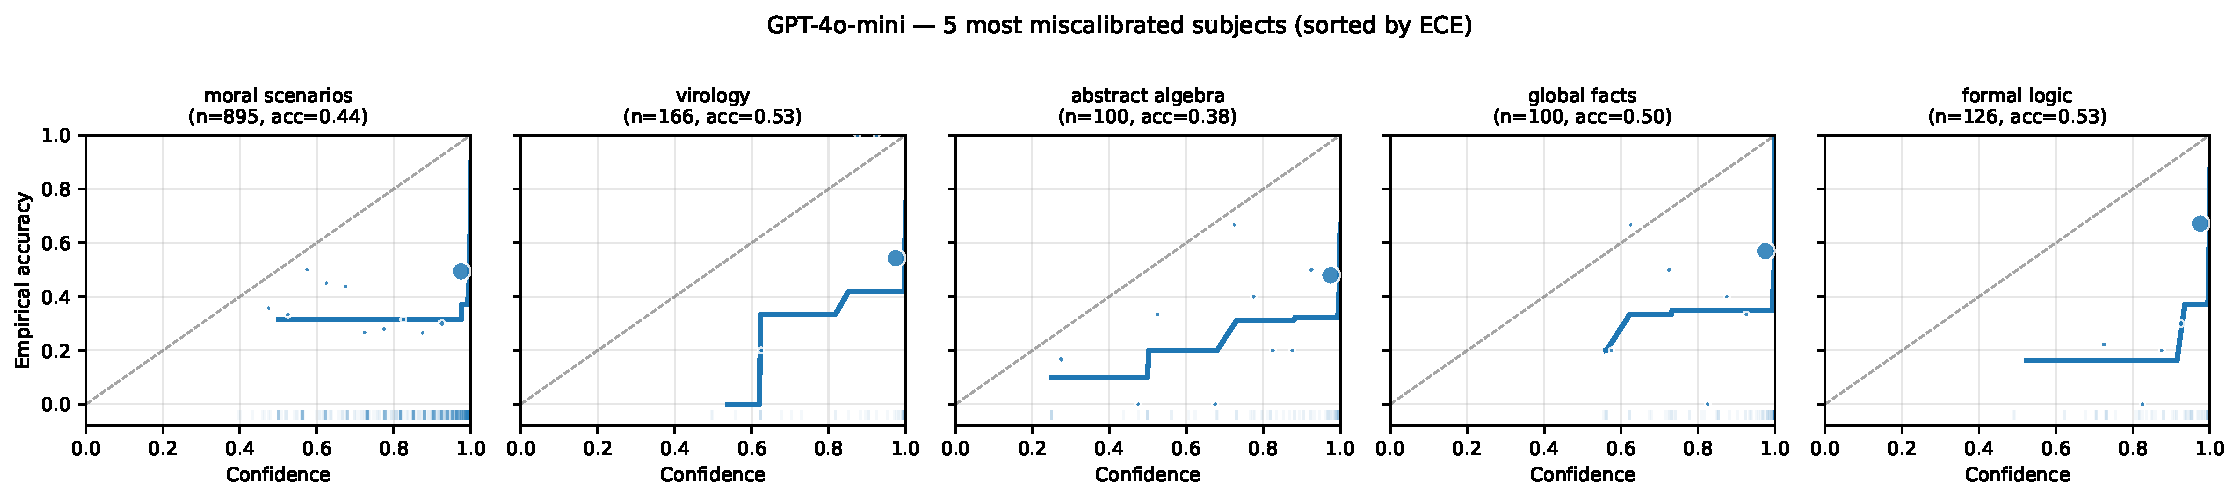
\includegraphics[width=\textwidth]{figures/top5_most_miscalibrated_gpt4o_4m.pdf}
  \caption{GPT-4o-mini reliability curves for the five most miscalibrated subjects
  by ECE. Solid line: isotonic regression fit, plotted only over the observed
  confidence range (1st--99th percentile per subject). Markers: empirical accuracy
  in 20 equal-width confidence bins, sized by bin count. The dashed line is the
  calibration diagonal. Annotations report sample size and mean accuracy.}
  \label{fig:top5}
\end{figure}

For visual contrast, Figure~\ref{fig:bottom5} shows the same plot for the five
\emph{best}-calibrated subjects for GPT-4o-mini. Curves there track the diagonal
closely or lie just below it; both shapes are present in the same model on the
same evaluation, illustrating the heterogeneity that aggregate ECE conceals.

\begin{figure}[h]
  \centering
  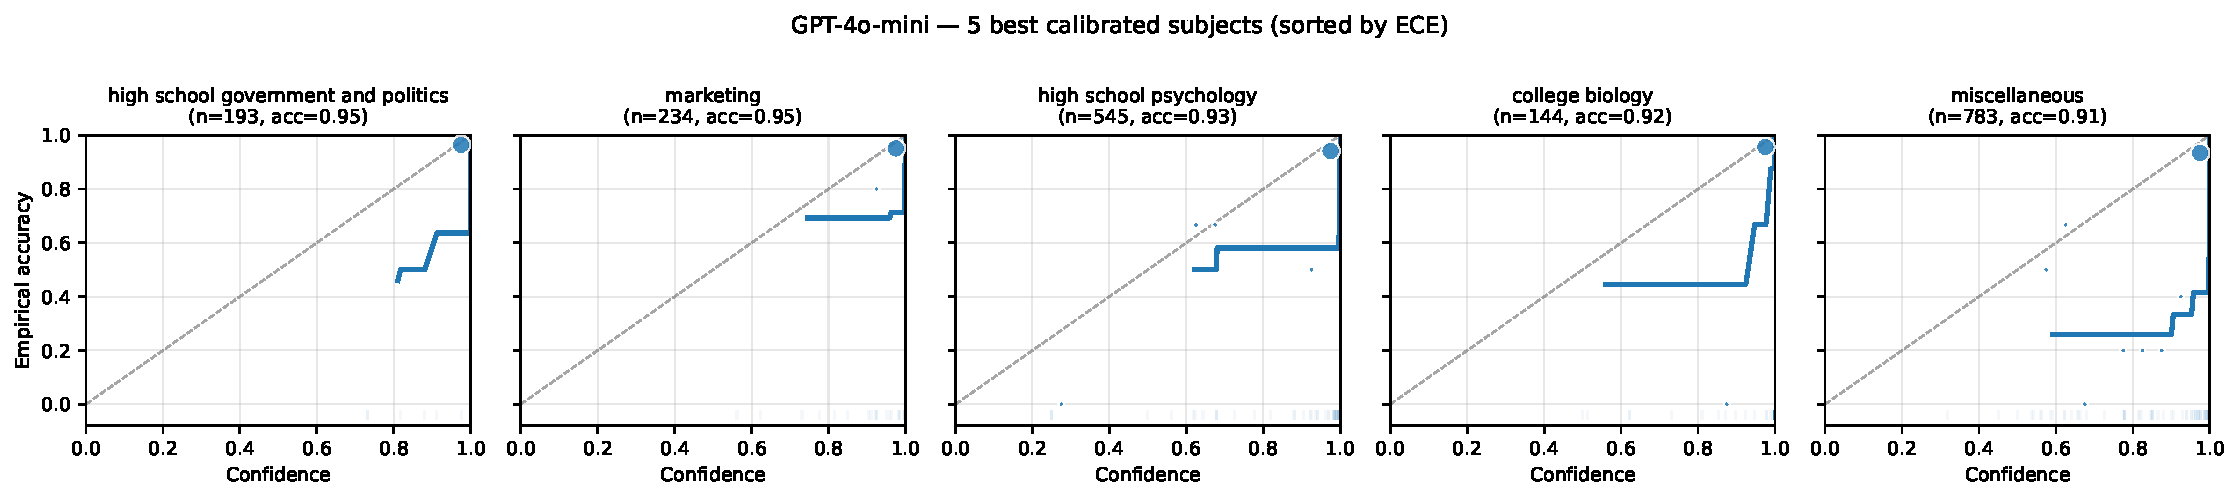
\includegraphics[width=\textwidth]{figures/bottom5_best_calibrated_gpt4o_4m.pdf}
  \caption{GPT-4o-mini reliability curves for the five \emph{best}-calibrated
  subjects, shown for visual contrast with Figure~\ref{fig:top5}. Same conventions.}
  \label{fig:bottom5}
\end{figure}

\subsection{Predictors of Miscalibration (RQ3)}

Table~\ref{tab:fixef} reports the fixed effects from the multilevel model
across all four models. The intercepts confirm large mean overconfidence in
every model, ranging from 0.157 (Qwen-1.5B) to 0.233 (Qwen-7B). Within the Qwen
family, the larger 7B model is \emph{more} overconfident than the smaller 1.5B
on average ($+49\%$ in the intercept), despite higher accuracy
(0.685 vs 0.536)---consistent with the documented effect of RLHF-style alignment
applied more aggressively to stronger base models
\citep{kadavath2022language, ouyang2022training, nakkiran2025trained}.

\begin{table}[h]
\centering
\caption{Fixed effects from the three-level mixed model for all four models.
Continuous covariates standardized. Significance: $^{***}p<0.001$,
$^{**}p<0.01$, $^*p<0.05$, $^\dagger p<0.10$.}
\label{tab:fixef}
\begin{tabular}{lrrrr}
\toprule
Predictor & GPT-4o-mini & Llama-Instruct & Qwen-1.5B-Instruct & Qwen-7B-Instruct \\
\midrule
Intercept         &  0.196$^{***}$ &  0.197$^{***}$ &  0.157$^{***}$ &  0.233$^{***}$ \\
Word count        &  0.031$^{***}$ & -0.005          &  0.004          &  0.019$^{**}$  \\
Max option length &  0.001          & -0.001          & -0.002          & -0.007          \\
Negation          & -0.001          &  0.007          & -0.010          & -0.001          \\
Entropy           &  0.016$^{***}$ &  0.008$^\dagger$ & -0.010$^{*}$    &  0.029$^{***}$ \\
\bottomrule
\end{tabular}
\end{table}

Figure~\ref{fig:coef} shows the corresponding forest plot. Word count is a
positive significant predictor for the two larger models (GPT-4o-mini, Qwen-7B)
and inert for the smaller two (Llama, Qwen-1.5B). The most informative pattern
is the entropy coefficient, which is positive for GPT-4o-mini ($+0.016$,
$p<0.001$) and Qwen-7B ($+0.029$, $p<0.001$), marginal for Llama
($+0.008$, $p=0.07$), and negative for Qwen-1.5B ($-0.010$, $p=0.02$).

\begin{figure}[h]
  \centering
  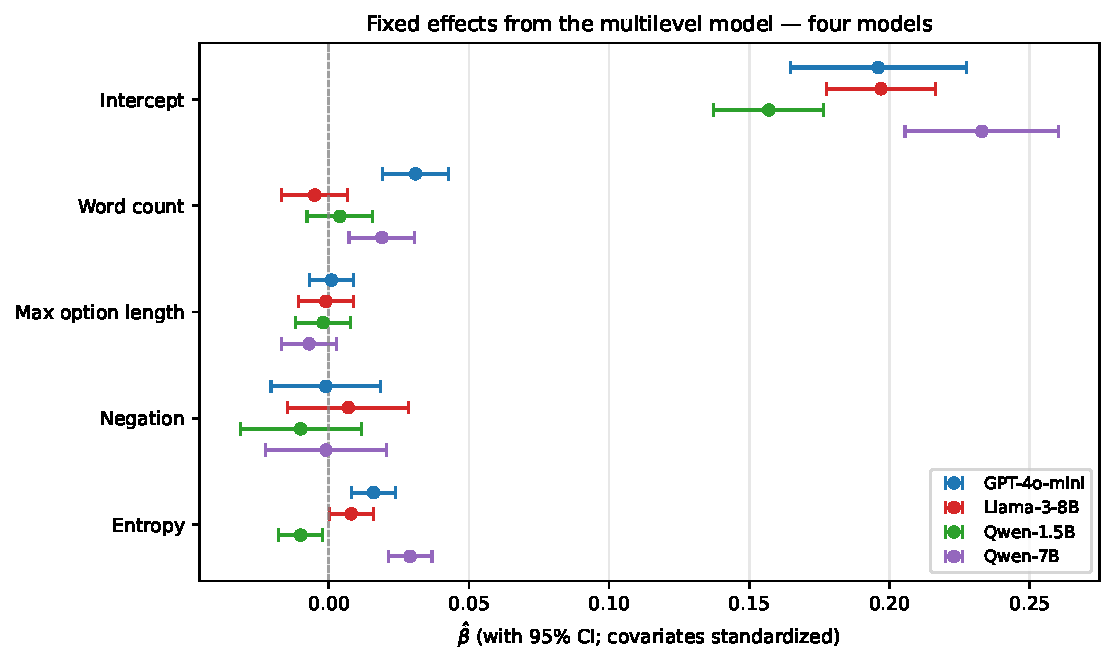
\includegraphics[width=0.85\textwidth]{figures/coef_plot_4m.pdf}
  \caption{Fixed effect estimates with 95\% confidence intervals for all four
  models. Estimates are on the standardized calibration gap scale.}
  \label{fig:coef}
\end{figure}

The entropy result is initially counterintuitive: higher option-distribution
entropy mechanically reduces top-1 confidence (the maximum probability over a
flatter distribution must be lower), so a naïve prediction is that high-entropy
questions should show \emph{smaller} calibration gaps. Figure~\ref{fig:entropy}
traces what is happening. Within each model, we partition questions into
entropy quartiles and report mean confidence (solid line) and mean accuracy
(dashed line) within each. As entropy rises, confidence does fall in all four
models, but in three of them accuracy falls \emph{faster}, so the gap (shaded
area) widens. Qwen-1.5B is the lone exception: its confidence and accuracy fall
in roughly parallel across the entropy range, which is exactly why its entropy
coefficient is negative.

\begin{figure}[h]
  \centering
  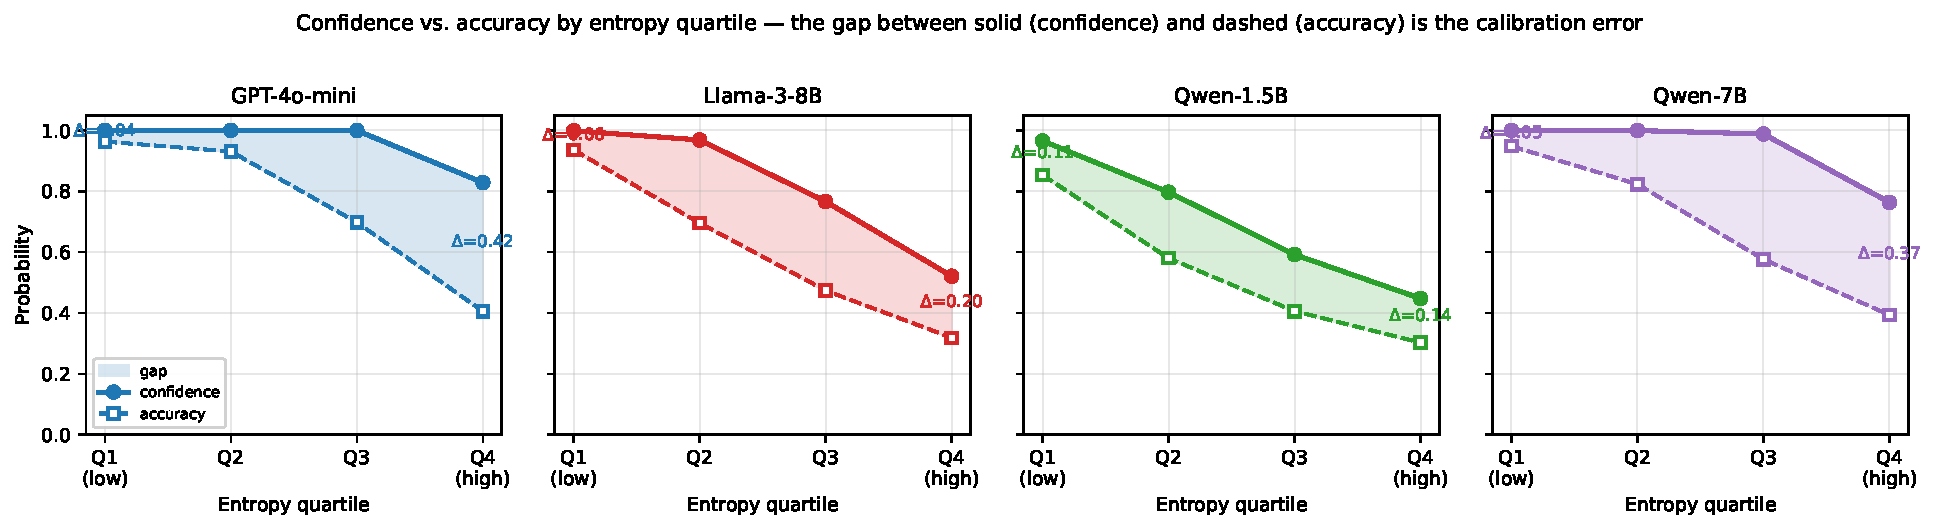
\includegraphics[width=\textwidth]{figures/entropy_mechanism_4m.pdf}
  \caption{Confidence (solid) and accuracy (dashed) by entropy quartile,
  per model. The shaded area is the calibration gap. Three of four models
  show confidence falling more slowly than accuracy, widening the gap; only
  Qwen-1.5B shows confidence and accuracy falling in parallel.}
  \label{fig:entropy}
\end{figure}

This marginal pattern is consistent with a literature on RLHF-induced confidence
saturation \citep{kadavath2022language, nakkiran2025trained, yaldiz2026balancing},
which finds at the aggregate level that instruction-tuned models maintain
high top-1 probability even when their option distribution suggests genuine
uncertainty. We are cautious about extending this further: the negative-coefficient
result rests on a single small-model checkpoint (Qwen-1.5B), and the
size differences between coefficients reflect observational rather than
controlled variation. Pending replication with additional small or base
models, our claim is descriptive: the four models we examine exhibit a sign
flip in the entropy coefficient that aligns with the direction prior literature
predicts.

\subsection{FDR-Corrected Subject Rankings}

Figure~\ref{fig:meangap} shows all 57 subjects sorted by mean calibration gap
for each model, with FDR-rejected subjects highlighted. At $\alpha=0.05$, all 57
subjects are rejected for GPT-4o-mini, Llama, and Qwen-7B; for Qwen-1.5B, 54 of
57 are rejected. The three subjects that fail to reject for Qwen-1.5B are
\texttt{high\_school\_government\_and\_politics} ($\bar{\text{gap}}=0.025$,
$p_{\text{adj}}=0.37$), \texttt{sociology} ($\bar{\text{gap}}=0.033$,
$p_{\text{adj}}=0.24$), and \texttt{us\_foreign\_policy}
($\bar{\text{gap}}=0.057$, $p_{\text{adj}}=0.14$). These are the only
subject-by-model cells in the entire 4-model $\times$ 57-subject study where
calibration is statistically indistinguishable from zero.

\begin{figure}[h]
  \centering
  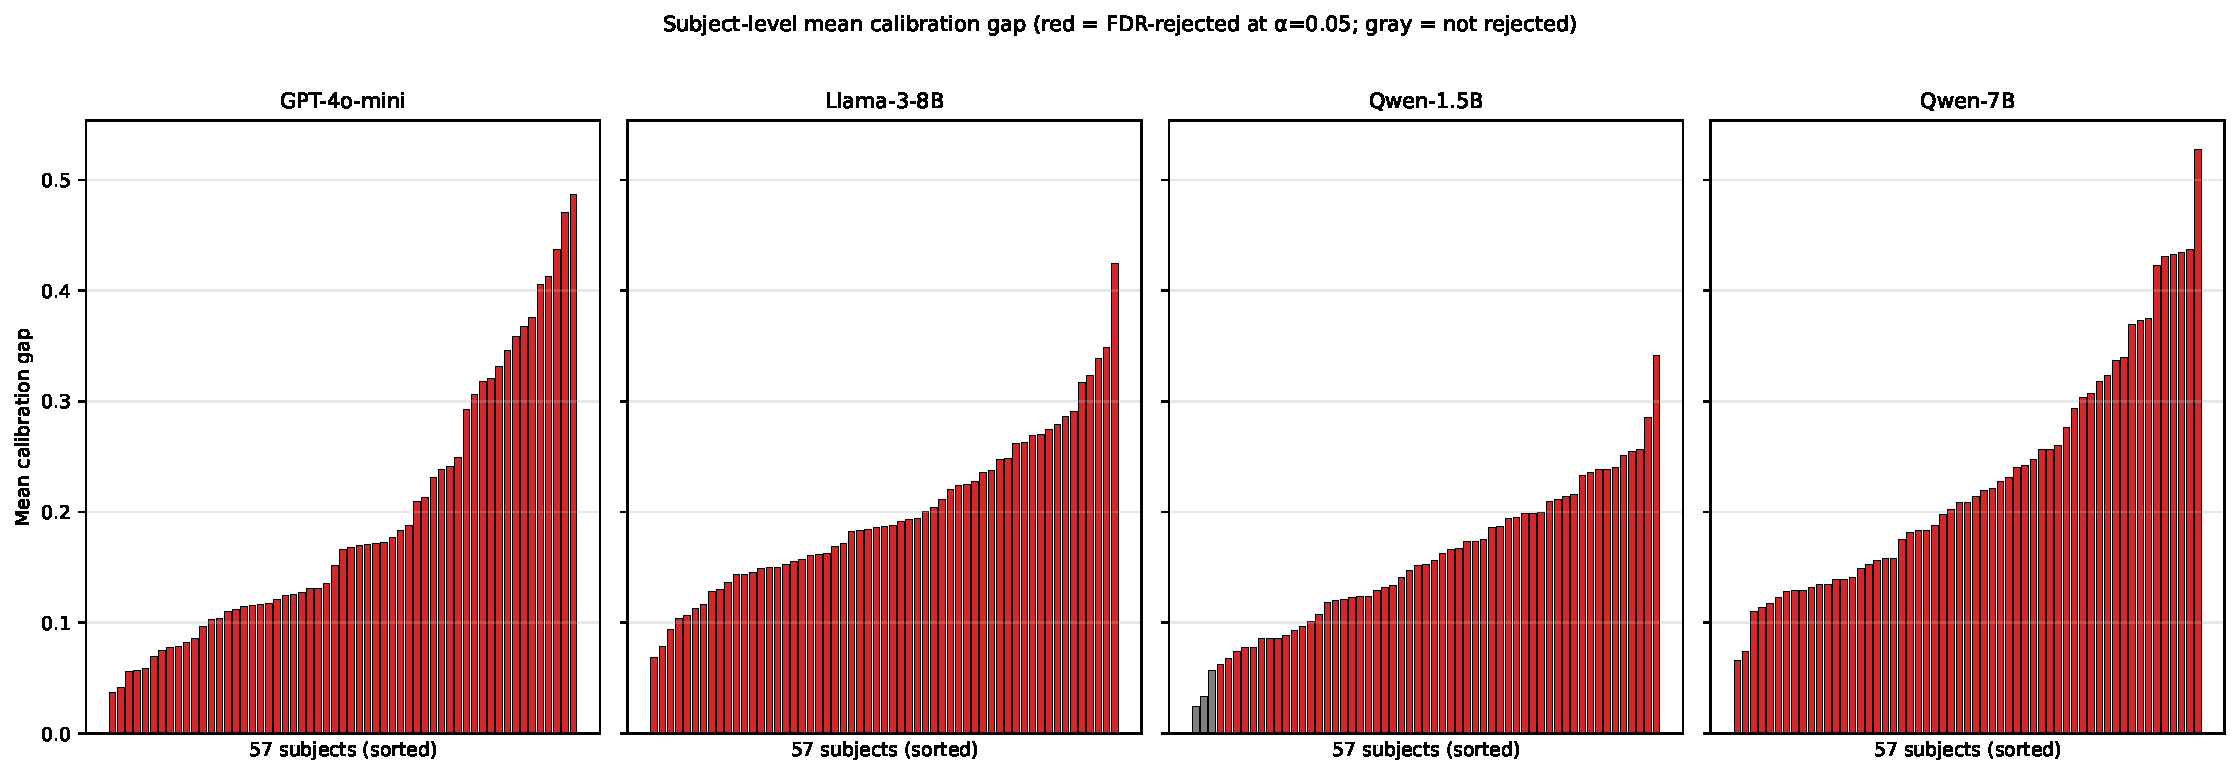
\includegraphics[width=\textwidth]{figures/subject_mean_gap_4m.pdf}
  \caption{Mean calibration gap per subject, sorted ascending. Red bars indicate
  subjects where $H_0$: mean gap $= 0$ is rejected at FDR $\alpha = 0.05$; gray
  bars are not rejected. Three of four models reject all 57 subjects; Qwen-1.5B
  rejects 54 of 57.}
  \label{fig:meangap}
\end{figure}

The substantive finding is therefore the \emph{magnitude} of heterogeneity, not
the binary reject/fail-to-reject outcome. Mean gaps span a 13.0$\times$ range
for GPT-4o-mini (0.037 to 0.487), 6.2$\times$ for Llama (0.069 to 0.425),
13.9$\times$ for Qwen-1.5B (0.025 to 0.342), and 8.0$\times$ for Qwen-7B
(0.066 to 0.527).

\paragraph{Subjects that are robustly worst-calibrated.} Across the four
models, the same subject clusters appear at the high-ECE end of the
distribution. Four subjects appear in the top-10 most miscalibrated for all
four models: \texttt{virology}, \texttt{college\_chemistry},
\texttt{college\_physics}, \texttt{professional\_law}. Expanding to top-15
adds \texttt{college\_mathematics}, \texttt{econometrics},
\texttt{high\_school\_physics}, \texttt{machine\_learning}, and
\texttt{moral\_scenarios}. These naturally cluster into three semantic groups:
(i) college-level quantitative STEM, (ii) niche factual recall (virology,
global facts), and (iii) structured ethical/legal reasoning (moral scenarios,
formal logic, professional law).

\paragraph{Subjects that are robustly best-calibrated.} Symmetric to the
above, the same subjects appear at the low-ECE end. The intersection of
bottom-5 ECE across all four models contains
\texttt{high\_school\_government\_and\_politics} and
\texttt{high\_school\_psychology}; bottom-10 adds
\texttt{high\_school\_us\_history}, \texttt{marketing}, and
\texttt{miscellaneous}; bottom-15 adds \texttt{high\_school\_geography},
\texttt{high\_school\_world\_history}, \texttt{sociology}, and
\texttt{us\_foreign\_policy}. Two patterns are visible. First, MMLU's
high-school-level subjects systematically show smaller calibration gaps than
their college-level counterparts; the level of specialization required appears
to track miscalibration. Second, well-calibrated subjects are dominated by
Social Sciences and the ``Other'' category (the applied/factual subjects in
the MMLU taxonomy)---no STEM subject appears in the bottom-10 intersection.
The audit recovers a coherent contrast: applied/factual high-school content is
where calibration is reliably good, and college-level technical content is
where it is reliably bad.

\subsection{Sensitivity Analysis}

Sensitivity-analysis conclusions extend uniformly across all four models. ECE
rankings are stable across bin counts (Spearman $\geq 0.97$ vs. the 20-bin
baseline for every model). The Negative Log Calibration Score, a strictly proper
scoring rule, ranks subjects nearly identically (Spearman $\geq 0.85$ across
models and bin counts). Two-level and three-level ICC estimates are numerically
identical, consistent with $\sigma^2_{\text{domain}}$ collapsing to zero.

The FDR-rejection finding is also robust to threshold choice for the three
larger models. At $\alpha = 0.01$, GPT-4o-mini rejects 56/57, Llama 55/57, and
Qwen-7B 57/57. Qwen-1.5B is more sensitive: at $\alpha = 0.01$, only 46 of 57
are rejected. This is consistent with Qwen-1.5B's lower mean intercept (0.157)
and broader distribution of subject-level $p$-values---the smallest model in
our set is the only one where many subjects' miscalibration is detectable but
not robust under the strictest FDR threshold.

\subsection{Cross-Model Agreement (RQ2)}

Figure~\ref{fig:crossmodel} shows the 4$\times$4 Spearman rank correlation
matrix for subject-level ECE across the four models. All six pairwise
correlations fall between 0.78 and 0.92. The cross-family pair GPT-4o-mini vs
Qwen-7B is the highest at 0.924, exceeding even the within-Qwen scaling
correlation (1.5B vs 7B, 0.849). Cross-family agreement at matched capability
is therefore stronger than within-family agreement across scale---the cleanest
evidence in our data that subject-level miscalibration is primarily a property
of the \emph{task} rather than of any particular model's training.

\begin{figure}[h]
  \centering
  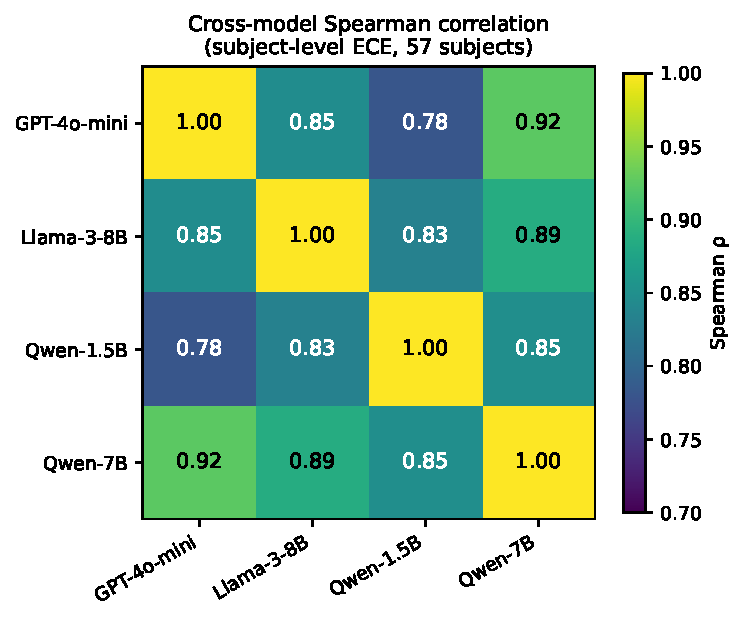
\includegraphics[width=0.55\textwidth]{figures/cross_model_heatmap_4m.pdf}
  \caption{Spearman rank correlation of subject-level ECE across the four models
  (57 common subjects). All pairwise correlations are in $[0.78, 0.92]$;
  bootstrap 95\% CIs are reported in the text.}
  \label{fig:crossmodel}
\end{figure}

Bootstrap 95\% confidence intervals (2000 replicates) for each pairwise
correlation are: GPT vs Llama $[0.73, 0.91]$, GPT vs Qwen-1.5B $[0.64, 0.87]$,
GPT vs Qwen-7B $[0.85, 0.96]$, Llama vs Qwen-1.5B $[0.73, 0.89]$, Llama vs
Qwen-7B $[0.80, 0.93]$, Qwen-1.5B vs Qwen-7B $[0.76, 0.90]$. None of these
intervals contains zero or even values close to it, and the lowest lower
bound (0.64) is still substantively large.

% ============================================================
\section{Discussion}
% ============================================================

\paragraph{Where calibration succeeds versus fails.}
The two strongest findings are descriptive but coherent. Calibration is
reliably good on high-school-level Social Sciences and applied/factual
subjects (\texttt{marketing}, \texttt{miscellaneous},
\texttt{high\_school\_government\_and\_politics},
\texttt{high\_school\_psychology}), and reliably bad on college-level
technical content (\texttt{college\_chemistry}, \texttt{college\_physics},
\texttt{college\_mathematics}, \texttt{machine\_learning}), niche factual
recall (\texttt{virology}, \texttt{global\_facts}), and structured
ethical/legal reasoning (\texttt{moral\_scenarios}, \texttt{professional\_law},
\texttt{formal\_logic}). The same patterns appear in every model we examined.
The level of specialization required appears to be a meaningful axis: MMLU's
high-school-level subjects consistently show smaller calibration gaps than
their college-level counterparts. This is the substantive finding the
heterogeneity audit recovers, and the kind of structure aggregate ECE conceals.

\paragraph{Cross-family agreement at matched capability.}
The Spearman correlation between GPT-4o-mini and Qwen-7B (0.924) exceeds the
within-family Qwen scaling correlation (0.849). All six pairwise correlations
fall in $[0.78, 0.92]$. Subject-level miscalibration is therefore more
consistent across model families at matched capability than within a single
family across scale---strong evidence that miscalibration patterns are
primarily a property of the task, not the model. This stability provides the
structural justification for choosing to scope corrections at the subject level
rather than globally; the targets of any such correction are stable across the
model space we examined, even though each correction would still be fit per
model on held-out data.

\paragraph{Within-family scale and entropy: descriptive observations.}
The Qwen 1.5B $\to$ 7B comparison shows the intercept rising from 0.157 to
0.233 ($+49\%$), ICC roughly tripling (0.019 $\to$ 0.049), and the entropy
coefficient flipping sign ($-0.010 \to +0.029$). All three changes go in the
same direction: more capable Qwen $\to$ more concentrated overconfidence. We
present this as an observation about the four checkpoints we measured rather
than a controlled scaling experiment. Figure~\ref{fig:entropy} traces the
entropy effect to a marginal pattern in which capable models maintain
near-saturated confidence even as the option distribution flattens, which is
consistent with prior literature on RLHF-induced confidence saturation
\citep{kadavath2022language, nakkiran2025trained, yaldiz2026balancing}. We
do not claim to have identified a causal mechanism; the comparison is between
checkpoints rather than a controlled within-checkpoint manipulation.

\paragraph{Implications for recalibration.}
Our framework is the diagnostic arm of a broader recalibration picture. The
operational arm has been studied directly: \citet{luo2025pretrained} fits
subject-specific temperature parameters per MMLU subject and demonstrates
improvements over a global correction. Our contribution is the upstream
question: is subject-level scoping a structurally appropriate choice in the
first place? The audit's affirmative answer---stable, cross-model targets with
robust statistical support---supplies that justification. Practitioners can
also reuse the audit findings as a transferable diagnostic test set: the
robustly worst-calibrated subjects we identify can flag miscalibration on a
new model before deployment, without re-running the full audit.

\paragraph{Limitations.}
Several limitations warrant caution. First, domain-level variance is estimated
at zero, likely because subject-level random effects absorb whatever
between-domain structure exists; with only four domain groups, power to detect
a separate domain component is very low, so we cannot cleanly partition
between-subject variance into domain-level and subject-within-domain
components. Second, the mixed model assumes homoskedastic residuals, which is
violated when calibration gap variance depends on per-subject accuracy. Third,
confidence is computed from logprobs at a single token position; this may not
faithfully represent the model's internal uncertainty, especially after RLHF
fine-tuning \citep{kadavath2022language}. Fourth, results are specific to
MMLU's four-choice format and may not generalize to open-ended generation
settings. Fifth, 4-bit quantization affects three of the four models studied
and may modestly attenuate confidence---most notably for Qwen-1.5B, whose
test-set accuracy (0.536) is below its published full-precision figure;
re-running this model under different precision settings would clarify how
much of its anomalous behavior (negative entropy coefficient, FDR robustness
gap) survives at full precision. Sixth, the entropy-coefficient sign comparison
rests on a single small-model checkpoint (Qwen-1.5B); replication with
additional small or base models---particularly within the Llama family---would
test whether the pattern is monotonic with capability or specific to that
checkpoint.

\paragraph{Future directions.}
Three directions extend the framework most directly. First, additional scale
points within the Qwen family (e.g., Qwen-2.5-14B) would let us fit a continuous
scaling relationship for the intercept and entropy coefficient rather than
contrasting two checkpoints. Second, adding a third model family (e.g.,
Mistral-7B or Gemma-2-9B at matched scale) would strengthen the cross-family
generalization claim from two families to three. Third, applying the framework
to MMLU-Pro or other harder benchmarks would test whether the
high-school-vs-college calibration gap we observe within MMLU persists at
higher difficulty levels.

% ============================================================
\section{Conclusion}
% ============================================================

We presented a statistical audit framework for LLM calibration heterogeneity
and applied it to MMLU using four instruction-tuned models from two families
across three parameter scales. The framework recovers a coherent contrast in
where calibration succeeds versus fails: applied/factual high-school subjects
are reliably well-calibrated, while college-level technical content, niche
factual recall, and structured ethical/legal reasoning are reliably bad.
Subject-level ECE rankings are highly correlated across all six model pairs
(Spearman $\rho \in [0.78, 0.92]$), with the cross-family GPT-4o-mini vs
Qwen-7B correlation being the highest. A within-family scale comparison
(Qwen-1.5B vs Qwen-7B) shows the intercept, between-subject ICC, and entropy
coefficient all changing in the direction prior aggregate literature
predicts---an observational pattern consistent with RLHF-induced confidence
saturation rather than a controlled mechanism test. The audit's stable targets
provide the structural justification for choosing subject-aware over global
recalibration scoping---a choice operationalized in concurrent work by
\citet{luo2025pretrained}---and supply a transferable diagnostic for flagging
miscalibration on new models before deployment.

% ============================================================
\section*{Statement of Work}
% ============================================================

\textbf{Data analysis.} Jennifer Zhang conducted the original two-model
analysis (GPT-4o-mini, Llama-3-8B-Instruct), including the multilevel model,
calibration curves, FDR correction, and sensitivity checks. John Wright
collected and analyzed the two additional Qwen-2.5 models, extended the
multilevel model and cross-model framework to four models, and produced the
within-family scale and entropy-mechanism analyses.
\textbf{Coding.} Jennifer Zhang built the original pipeline; John Wright
extended it to support arbitrary models and produced the parameterized
inference notebook used for the open-weight models.
\textbf{Writing.} Jennifer Zhang drafted the original report; John Wright
revised it for the four-model expansion and produced the final manuscript.
\textbf{Presentation.} Jennifer Zhang prepared the original slide deck.

% ============================================================
\bibliographystyle{plainnat}
\bibliography{references}
% ============================================================

\end{document}
